\documentclass{beamer}
\usepackage{listings}
\usepackage{hyperref}
\usepackage{graphicx}
\usetheme{Antibes}

\title[Introduction to Python]{Introduction to Python for Scientists}
\author{Imreh Gergely}
\institute{IAMS}
\date{2009 October 15}

\lstset{ %
language=Python,                % choose the language of the code
basicstyle=\footnotesize,       % the size of the fonts that are used for the code
% numbers=left,                   % where to put the line-numbers
% numberstyle=\footnotesize,      % the size of the fonts that are used for the line-numbers
% stepnumber=2,                   % the step between two line-numbers. If it's 1 each line will be numbered
% numbersep=5pt,                  % how far the line-numbers are from the code
% backgroundcolor=\color{white},  % choose the background color. You must add \usepackage{color}
showspaces=false,               % show spaces adding particular underscores
showstringspaces=false,         % underline spaces within strings
showtabs=false,                 % show tabs within strings adding particular underscores
frame=single,	                % adds a frame around the code
tabsize=2,	                % sets default tabsize to 2 spaces
captionpos=b,                   % sets the caption-position to bottom
breaklines=true,                % sets automatic line breaking
breakatwhitespace=false,        % sets if automatic breaks should only happen at whitespace
escapeinside={\%*}{*)}          % if you want to add a comment within your code
}

\begin{document}

\begin{frame}
\titlepage
\end{frame}

\begin{frame}
\frametitle{Today's program}
\tableofcontents
\end{frame}

\section{"Hello World"}
\begin{frame}[fragile]
  \frametitle{Your first Python program}
  \begin{itemize}[<+->]
    \item Here it is:
\lstinputlisting{code/example01.py}
  	\item Using the Python console
  	\item Using a program editor
  \end{itemize}
\end{frame}

\section{Functions / Subroutines}
\begin{frame}[fragile]
  \begin{block}{Functions are your friend}
	 \begin{itemize}[<+->]
		 \item Use function if you want to repeat a calculation
		 \item Named functions:
\begin{lstlisting}
def function_name(parameters):
    ''' Function description '''
    result = (...do something...)
    return result
\end{lstlisting}
		 \item "Anonymous" functions
\begin{lstlisting}
f = lamda parameters: (...do something...)
\end{lstlisting}
		 \item Be careful of indentations!
	 \end{itemize}
  \end{block}
\end{frame}

\begin{frame}[fragile]
  \frametitle{Importing functions from modules}
  \begin{block}{Where you can, use functions that already exist}
	 \begin{itemize}[<+->]
		 \item Import all functions from a module version 1:
\begin{lstlisting}
import scipy
x = scipy.exp(0)
\end{lstlisting}
		 \item Import all functions from a module version 2:
\begin{lstlisting}
from scipy import *
x = exp(0)
\end{lstlisting}
		 \item Import selected functions from a module:
\begin{lstlisting}
from scipy import exp
x = exp(0)
\end{lstlisting}
	 \end{itemize}
  \end{block}
\end{frame}

\section{Plotting}
\subsection{Loading data files}
\begin{frame}[fragile]
  \begin{block}{Many ways to load a data file, this is one}
  You can use a function from the \textbf{numpy} package:
\begin{lstlisting}
from numpy import loadtxt
data = loadtxt(filename, ...)
\end{lstlisting}
  Commonly used parameters are: delimiters, skiprows, columns...
  \end{block}
\end{frame}

\subsection{Show the data}
\begin{frame}[fragile]
	\frametitle{Simple plotting}
Very simple plotting is done with the \textbf{matplotlib / pylab} package.
\begin{lstlisting}
import pylab
pylab.plot(x, y)
pylab.show()
\end{lstlisting}
\begin{figure}[htp]
\centering
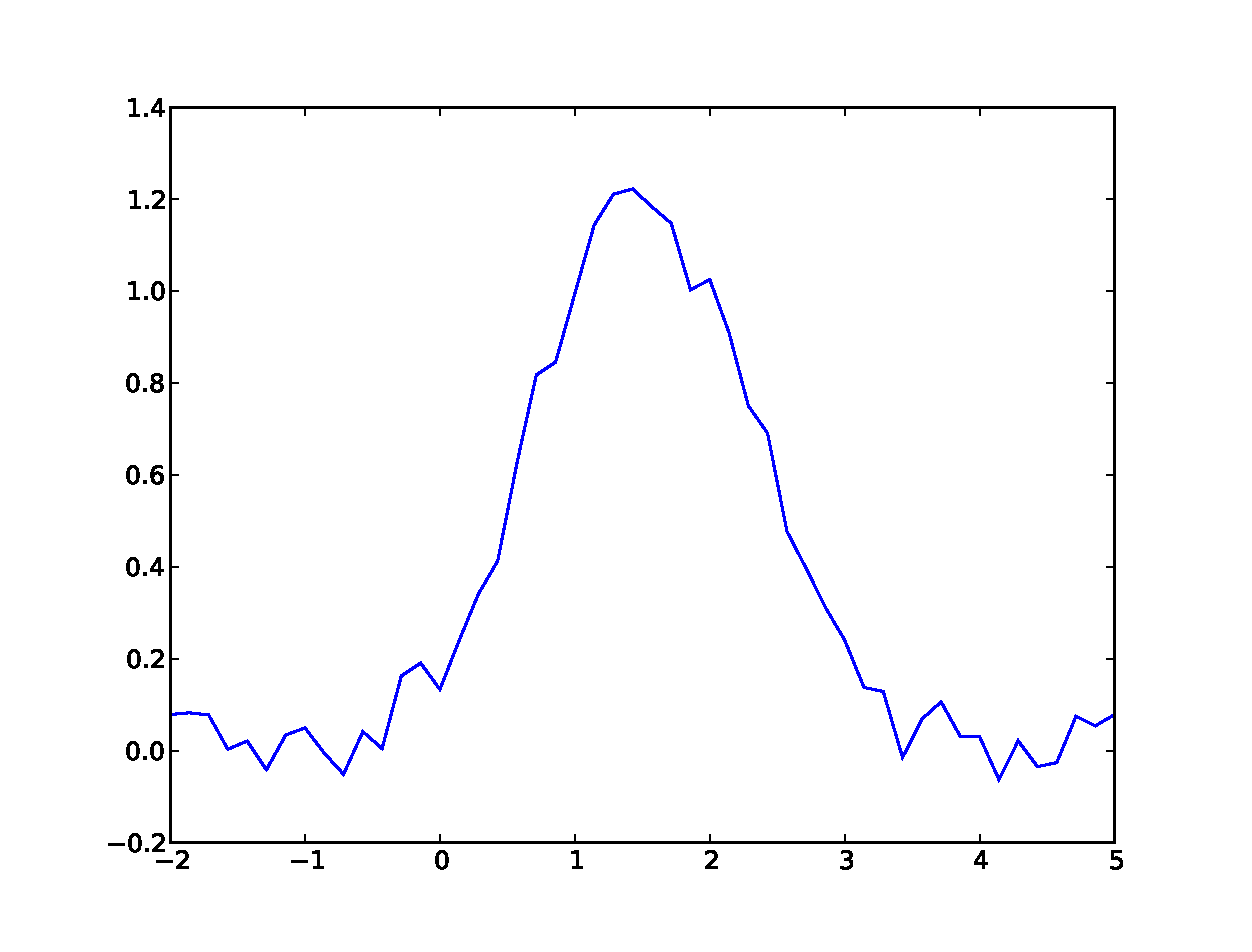
\includegraphics[width=6cm]{code/example02}
\end{figure}
\end{frame}


\begin{frame}[fragile]
	\frametitle{Real datafile}
Real data file from Tektronix oscilloscope
\uncover<2>{
\begin{figure}[htp]
\centering
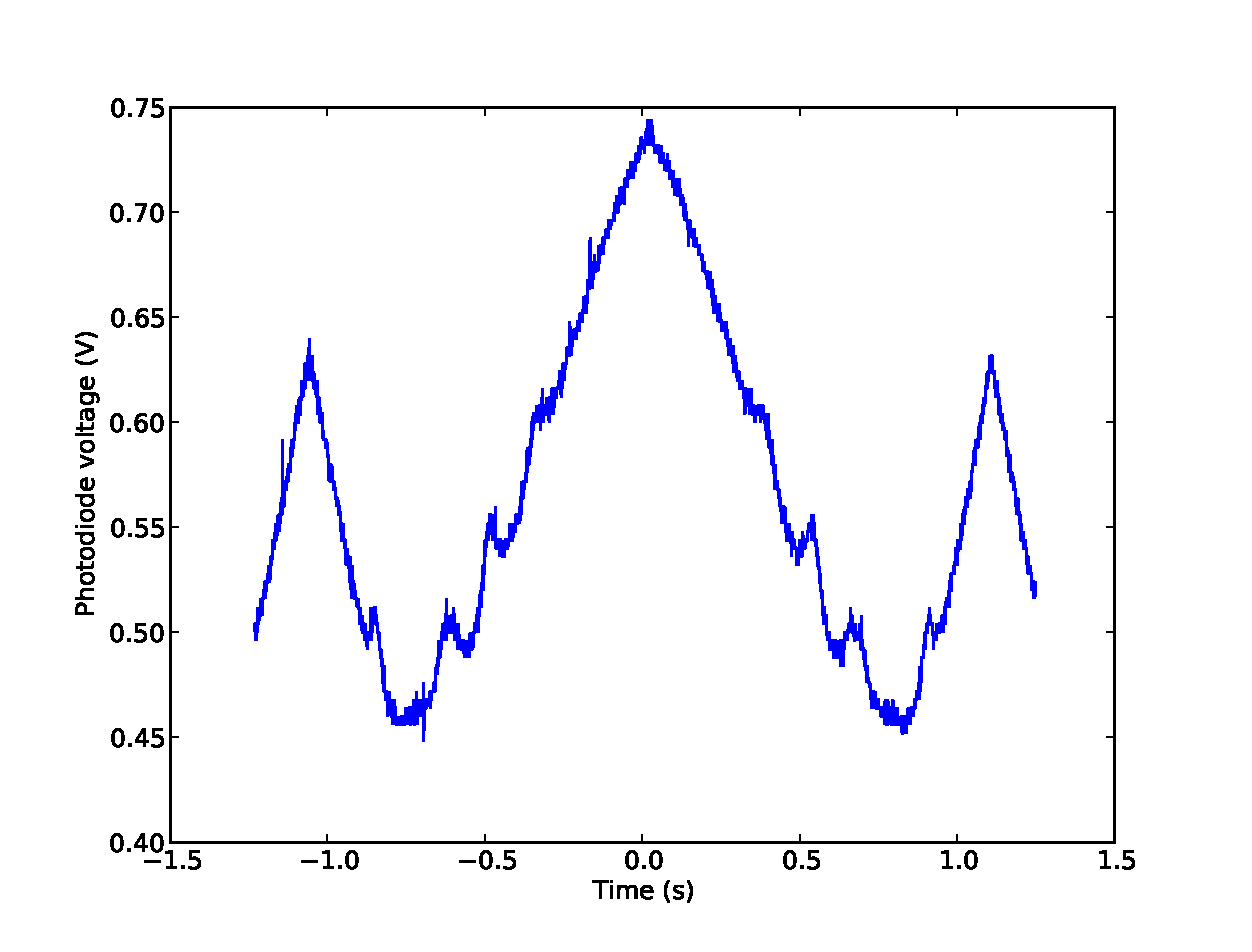
\includegraphics[width=8cm]{code/oscilloscope}
\end{figure}
}
\end{frame}


\begin{frame}[fragile]
	\frametitle{Formatting}
Simple formatting by including format string:
\begin{lstlisting}
pylab.plot(x, y, "b.")
\end{lstlisting}
\begin{figure}[htp]
\centering
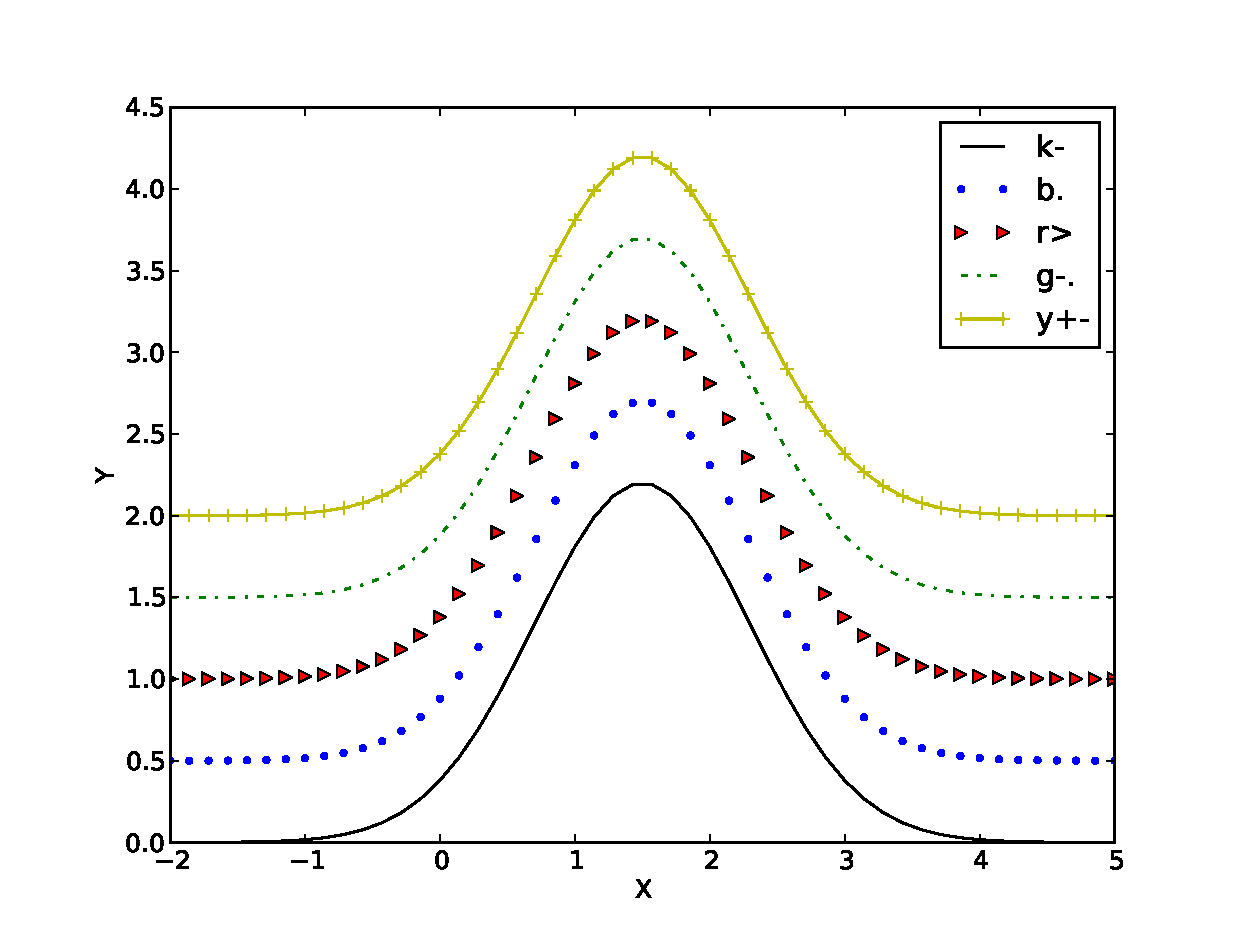
\includegraphics[width=7cm]{code/formatting}
\end{figure}
\end{frame}

\section{Fitting}
\begin{frame}[fragile]
  \frametitle{Fitting}
  \begin{block}{Data fitting steps}
	 \begin{itemize}[<+->]
		 \item Define fitted function
		 \item Create error-function
\begin{lstlisting}
err = lambda p, x, y: model(p, x) - y
\end{lstlisting}
		 \item Load data
		 \item Choose starting paramters
		 \item Do fitting: minimize error function
\begin{lstlisting}
from scipy import optimize
p1,success = optimize.leastsq(err, p0, args=(x, y))
\end{lstlisting}
		 \item Plot results and print parameters
	 \end{itemize}
  \end{block}
\end{frame}


\section{Now you try it...}
\subsection{Generate data}
\begin{frame}[fragile]
  \frametitle{Generate data}
  \begin{block}{Fitting challenge}
	 \begin{itemize}[<+->]
		 \item Choose some function with 3-4 tunable parameters
		 \item Generate data with that function
		 \item add noise: 
\begin{lstlisting}
y = function(p, x) + rand(num_points)
\end{lstlisting}
	 \end{itemize}
  \end{block}
\end{frame}

\subsection{Shuffle and fit}
\begin{frame}
  \frametitle{Shuffle and fit}
  \begin{block}{Fitting challenge}
	 \begin{itemize}[<+->]
		 \item Give your example data to someone else
		 \item Take someone else's data
		 \item Fit it
		 \item Check whether you got the right parameters
	 \end{itemize}
  \end{block}
\end{frame}

\section{Useful things}
\begin{frame}[fragile]
  \frametitle{Useful things}
  \begin{block}{Commonly used other things}
	 \begin{itemize}[<+->]
		 \item Loop:
\begin{lstlisting}
for i in range(0, 10):
    print i
\end{lstlisting}
		 \item Conditional:
\begin{lstlisting}
if (x > 10):
   print "X is too large!"
\end{lstlisting}
	 \end{itemize}
  \end{block}
\end{frame}

\section{Homework}
\begin{frame}
  \frametitle{Homework}
  \begin{block}{Practice this on your own}
  Find some data that you analyzed previously and redo it with Python.
  \end{block}
\end{frame}

\begin{frame}
  \frametitle{More knowledge}
  \begin{block}{There are a lot of sources of information on the Web}
   \begin{itemize}
    \item Python documentation \url{http://docs.python.org/}
   	\item Scipy/Numpy documentation \url{http://docs.scipy.org/doc/}
   	\item Scipy Cookbook with examples \url{http://www.scipy.org/Cookbook}
   	\item Matplotlib, examples \& gallery \url{http://matplotlib.sourceforge.net/}
   	\item Google Code Search \url{http://www.google.com.tw/codesearch}
   	\item ...many more...
   \end{itemize}
  \end{block}
\end{frame}


\end{document}
